\chapter{Gene Expression Programming}\label{chapter:gep}
This chapter explores the foundational principles of GEP, its integration with neural networks through gene expression programming neural networks, and current research, highlighting GEP's role as a transformative tool in computational intelligence. An introduction to GEP is given in Section \ref{sec:gep_introduction}, after which the historical background is discussed in Section \ref{sec:gep_historical_background}. Section \ref{sec:gep_core_concepts} provides the reader with the fundamental mechanics behind GEP and it's neural network extension, GEP-NN. The strengths and challenges of GEP are discussed in Section \ref{sec:gep_strenght_challenges} and finally, Section \ref{sec:gep_current_research} summarizes recent advancements made in GEP and GEP-NN.


\section{Introduction}\label{sec:gep_introduction}
Gene Expression Programming (GEP) is an evolutionary algorithm that blends the strengths of genetic programming and genetic algorithms seen in Chapter \ref{chapter_ea} in order to solve complex computational problems. Introduced by Candida Ferreira in 2001, GEP is distinguished by its unique encoding method which decouples the genotype (fixed-length chromosome) from the phenotype (expression trees) (\cite{ferreira2006gene}). This dual representation enables the efficiency and versatility that GEP brings, enabling it to explore complex solution spaces with a balance of exploration and exploitation.

\parbreak\noindent In GEP, candidate solution are represented as fixed length linear chromosomes composed of genes, which are later translated into function programs or expressions. This genotype-to-phenotype mapping is powered by Karva notation and allows GEP to maintain the structural integrity of solutions during  genetic operators like crossover and mutation, addressing the key limitation in genetic programming where such genetic operations often disrupt and result in non-functional expressions.

\parbreak\noindent GEP generally excels in tasks requiring symbolic regression, optimization, and automated problem-solving. It has been used in applications ranging from classification problems (CP) to automatic model design problems (AMDP) (\cite{zhong2017gene}). One of its most innovative applications is in the creation of neural networks using GEP-NN. Gene Expression Programming Neural Networks (GEP-NN) is an extension on GEP whereby the topology and weights of a neural network are evolved using the principles of GEP. The neural network is encoded in three separate domain, namely, the normal GEP genotype domain representing the nodes of the neural net, and two additional domains, \textit{Dw} and \textit{Dt} which encode the weight connection and threshold values respectively (\cite{ferreira2006gene}).

\section{Historical Development of GEP}\label{sec:gep_historical_background}
The origins of Gene Expression Programming (GEP) can be traced to Candida Ferreira's groundbreaking in the early 2000s (\cite{ferreira2006gene}). In attempt to overcome the limitations of genetic algorithms (GA) and genetic programming (GP), Ferreira introduced GEP in 2001 as a novel evolutionary approach that decoupled the representation of solutions in their genotype form from their phenotype functional expression representation. The introduction of this algorithm addressed challenges such as inefficiencies in genetic operations and the difficulty of evolving structurally complex solutions. This established GEP as a versatile tool for solving a wide range of optimization problems (\cite{ferreira2006gene}).

\parbreak\noindent Ferreira's development of GEP was motivated by limitations of GP, particularly the disruption of functional expressions during evolutionary genetic operators such as crossover and mutation. By encoding solutions as fixed-length linear chromosome, GEP ensured that when these genetic operations were applied, it would not compromise the integrity of functional structures. These chromosomes were then expressed in their phenotype form as parse trees or directed graphs, showcasing its genotype-phenotype mapping flexibility (\cite{ferreira2006gene}).

\parbreak\noindent The publication of Ferreira's book, \textit{Gene Expression Programming: Mathematical Modeling by an Artificial Intelligence}, in 2001 sparked interest in the broader research community. Early experiments demonstrated GEP's superiority in tasks such as symbolic regressions, where it outperformed competing optimization algorithms by producing simpler, more interpretable solutions.

\parbreak\noindent By the mid-2000s, GEP was integrated with neural networks to optimize topology and weights, giving rise to gene expression programming neural networks (GEP-NN). This marked a significant advancement, as GEP's ability to evolve the entire architecture established it as a powerful alternative to traditional training methods like backpropagation (\cite{ferreira2006gene}).

\parbreak\noindent Initially focused on symbolic regressions, GEP quickly found applications in other fields such as engineering and medicine (\cite{malik2016application}, \cite{kusy2013application}). Researchers began adapting GEP to solve multi-objective problems and handle dynamic environments, broadening its usage (\cite{zheng2012multi}). Today, GEP is recognized as a versatile and scalable evolutionary algorithm and has been seen to be used in many other fields such as the optimization of blasting patterns in mines (\cite{bayat2022blasting}), and its usage in predicting pavement performance, an essential metric used in the rehabilitation and reconstruction of roads (\cite{mazari2016prediction}).

\section{Core Concepts in Gene Expression Programming}\label{sec:gep_core_concepts}

\begin{figure}[H] % Use [H] to suppress floating and place the figure/table exactly where it is specified in the text
	\centering % Horizontally center the figure on the page
	\includesvg[width=\textwidth]{Figures/chapter_gep/gep_algorithm.svg} % Include the figure image
	\caption{Gene Expression Programming Algorithm (adapted from \cite{ferreira2006gene})}
	\label{fig:gep_algorithm} % Unique label used for referencing the figure in-text
\end{figure}

\parbreak Gene Expression Programming (GEP) is defined by its unique approach to encoding solutions, translating genetic representations into guaranteed functional outputs, and employing a suite of genetic operators to evolve populations over successive generations mimicking evolutionary processes. Understanding these core concepts is essential in grasping the algorithm that this paper proposes. The basic GEP algorithm can be summarised as shown in Figure \ref{fig:gep_algorithm}.

\subsection{The Genome}
\subsubsection{GEP}
Understanding how GEP works begins with understanding how the genome is constructed. The chromosome is a linear fixed-length string made up of symbols (genes). The chromosome represents the genotype, and can then be decoded to represent the expression tree which is the phenotype (\cite{ferreira2006gene}). For example, consider the following algebraic expression:
\begin{ceqn}
    \begin{equation}\label{alg:gep_chromsome_example}
        \sqrt{(a \times b) + c}
    \end{equation}
\end{ceqn}

\parbreak\noindent This equation can be represented as an expression tree seen in Figure \ref{alg:gep_chromsome_example}, representing the phenotype, where $Q$ represents the square root function.

\parbreak\noindent GEP makes use of \textit{Karva Notation} as a genotype-phenotype mapping scheme which maps an expression tree into a \textit{K-expression}. It works by simply reading the expression tree left-to-right and top-to-bottom. The expression tree seen in Figure \ref{alg:gep_chromsome_example} can then be represented in its genotype form (K-expression) as follows:
\begin{ceqn}
\begin{equation}
    \begin{array}{cccccc}
        0 & 1 & 2 & 3 & 4 & 5\\
        Q & + & \times & c & a & b
    \end{array}
\end{equation}
\end{ceqn}

\parbreak
\begin{figure}[H] % Use [H] to suppress floating and place the figure/table exactly where it is specified in the text
	\centering % Horizontally center the figure on the page
	\includesvg[width=0.3\textwidth]{Figures/chapter_gep/chapter_gep_phenotype.svg} % Include the figure image
	\caption{Example Expression Tree For Mathematical Equation \ref{alg:gep_chromsome_example}}
	\label{fig:gep_phenotype_example} % Unique label used for referencing the figure in-text
\end{figure}
  
\parbreak\noindent Although GEP primarily uses k-expressions as its mapping scheme, postfix and prefix configurations exist - using the expression tree in Figure \ref{fig:gep_phenotype_example}, postfix would be encoded as seen in Equation \ref{alg:postfix}, and prefix would be encoded as seen in Equation \ref{alg:prefix}.
\begin{ceqn}
    \begin{equation}\label{alg:postfix}
        \begin{array}{cccccc}
            0 & 1 & 2 & 3 & 4 & 5\\
            a & b & \times & c & + & Q
        \end{array}
    \end{equation}
\end{ceqn}

\begin{ceqn}
    \begin{equation}\label{alg:prefix}
        \begin{array}{cccccc}
            0 & 1 & 2 & 3 & 4 & 5\\
            Q & + & \times & a & b & c
        \end{array}
    \end{equation}
\end{ceqn}

\subsubsection{GEP-NN}
\noindent As mentioned, GEP extends its methodology to encode and evolve neural networks due to its simplicity and plasticity. The general neural network seen in Section \ref{sec:nn_nutshell} can be easily translated in an expression tree as shown in Figure \ref{fig:gep_nn_example} where \textit{a} and \textit{b} represents the inputs \textit{i1} and \textit{i2} respectively, and \textit{D} represents a function with connectivity two which serves as the weighted sum (\cite{ferreira2006gene}).

\begin{figure}[H] % Use [H] to suppress floating and place the figure/table exactly where it is specified in the text
	\centering % Horizontally center the figure on the page
	\includesvg[width=0.8\textwidth]{Figures/chapter_gep/chapter_gep_nn_example.svg} % Include the figure image
	\caption{Example Neural Network and its Expression Tree Counterpart}
	\label{fig:gep_nn_example} % Unique label used for referencing the figure in-text
\end{figure}

\subsection{Structural Organization of Genes}
\subsubsection{GEP}
GEP genes are composed of two different domains, namely, the head and the tail. The head domain is used to encode the function symbols used in the optimization problem while the tail serves as a buffer of terminal symbols in order to guarantee that functional expression trees are generated. The length of the genome is made up of the head and the tail. It should be noted that the head can contain both function symbols and terminal symbols. The length of the head is predefined, and the tail is calculated as follows (\cite{ferreira2006gene}):
\begin{ceqn}
    \begin{equation}\label{alg:prefix}
        t = h \times (n_{max} - 1) + 1
    \end{equation}
\end{ceqn}

\noindent where:
\begin{itemize}
    \item \textbf{$t$} is the length of the tail
    \item \textbf{$h$} is the length of the head (predefined)
    \item \textbf{$n_{max}$} is the number of arguments of the function with the most arguments (also called the maximum arity)
\end{itemize}

\parbreak\noindent As an example with reference to the expression to mathematical Equation \ref{alg:gep_chromsome_example}, the function set would be $F=\{Q,\times,+\}$ and the terminal set would be $T=\{a,b,c\}$. The maximum arity $n_{max}$ would be 2 as multiplication and addition both take in two arguments (as opposed to Q/square root which takes one argument). Provided a head size of 4 was chosen, the tail length would then be $t = 4 \times (2 - 1) + 1 = 5$. The chromosome length would as a result be $h + t = 4 + 5 = 9$. A chromosome representing Equation \ref{alg:gep_chromsome_example} could look as follows (tail is in bold):
\begin{ceqn}
    \begin{equation}\label{alg:gep_full_chromosome}
        \begin{array}{ccccccccc}
            0 & 1 & 2 & 3 & 4 & 5 & 6 & 7 & 8\\
            Q & + & \times & a & \textbf{b} & \textbf{c} & \textbf{a} & \textbf{b} & \textbf{a}
        \end{array}
    \end{equation}
\end{ceqn}

\parbreak\noindent The tail acts like a reservoir of terminal symbols meaning that functional expression trees are always a given. Not all terminal symbols are guaranteed to be used in the phenotype representation - those symbols that are not used are referred to as the non-coding region, whilst the symbols that are used is referred as the coding region (\cite{ferreira2006gene}).

\parbreak\noindent GEP chromosomes do not necessarily need to contain only one gene - multigenic systems can easily be represented, for example:
\begin{ceqn}
    \begin{equation}\label{alg:gep_full_chromosome}
        \begin{array}{cccccccccccccccccc}
            0 & 1 & 2 & 3 & 4 & 5 & 6 & 7 & 8 & 9 & 0 & 1 & 2 & 3 & 4 & 5 & 6 & 7 \\
            Q & + & \times & a & \textbf{b} & \textbf{c} & \textbf{a} & \textbf{b} & \textbf{a} & + & + & Q & b & \textbf{a} & \textbf{a} & \textbf{b} & \textbf{c} & \textbf{a}
        \end{array}
    \end{equation}
\end{ceqn}

\parbreak\noindent These two genes represent two respective sub-expression trees. By incorporating mutligenic systems, complex genomes can be created by smaller genomes, a common occurrence seen in nature (\cite{ferreira2006gene}). For optimization problems with multiple outputs such as classification problems, the different sub-expression trees are seen as autonomous agents working together to each produce a particular output for a set of given inputs (\cite{ferreira2006gene}). Sub-expression trees can also be combined using a linking function to form a larger expression tree as shown in Figure \ref{fig:gep_linking_function} (using Equation \ref{alg:gep_full_chromosome}). Multigenic chromosomes guide the evolution in modular structures, a small building block in order to create more complex structure.

\parbreak
\begin{figure}[H] % Use [H] to suppress floating and place the figure/table exactly where it is specified in the text
	\centering % Horizontally center the figure on the page
	\includesvg[width=\textwidth]{Figures/chapter_gep/chapter_gep_linking.svg} % Include the figure image
	\caption{Example of Linking Function to Connect Sub Expression Trees}
	\label{fig:gep_linking_function} % Unique label used for referencing the figure in-text
\end{figure}

\subsubsection{GEP-NN}
When using GEP genomes to represent neural networks, two additional domains are required in order to encode the weights of the connectivities between nodes, and the thresholds used when applying an activation function (\cite{ferreira2006gene}). These two domains, denoted, \textit{Dw} and \textit{Dt}, are encoded in their own regions within the chromosome. Depending on the problem at hand in which a neural network needs to be designed for, these additional domains are characterized by the outcome. In some instances, the threshold domain is not required, especially when using activation functions that are non-linear. The chromosome for the expression tree seen in Figure \ref{fig:gep_nn_example} would look as follows:
\begin{ceqn}
    \begin{equation}\label{alg:gep__nn_chromosome_example}
        \begin{array}{cccccccccccccccccc}
            0 & 1 & 2 & 3 & 4 & 5 & 6 & 7 & 8 & 9 & 0 & 1 & 2 \\
            D & D & D & a & b & a & b & \textbf{1} & \textbf{2} & \textbf{3} & \textbf{4} & \textbf{5} & \textbf{6} &
        \end{array}
    \end{equation}
\end{ceqn}

\noindent where position 0 to 6 represents the neural network gene region, and the positions in bold are the weights. Typically, the \textit{Dw} gene stores indices and is used to fetch indices from a lookup array as necessary. This array could look as \textit{$W = \{-1.2, 0.8, -0.3, 1.4, 0.5, -2.0\}$}. The length of the \textit{Dw} domain is calculated using \textit{$Dw_{length} = h \times n_{max}$} and the length of \textit{Dt} is calculated using \textit{$Dt_{length} = h$} (\cite{ferreira2006gene}).


\subsection{Genotype Operators}\label{sec:gep_genetic_operators}
GEP employs a variety of genetic operators to balance exploration and exploitation. These operators are tailored to its fixed-length genotype and ensure syntactically correct phenotypes. These genetic operators are modified in various ways to extend its application in the GEP-NN domain.

\subsubsection{Mutation}
Mutation in GEP is one of the most efficient genetic operators allowing candidate solutions to adapt very quickly. For a given mutation $p_m$, two one-mutations operations are applied to the chromosome. If the mutation point happens to be in the head, the mutation can result in symbols from both the function and terminal set whereas if it occurs in the tail, only symbols from the terminal set can be chosen (\cite{ferreira2006gene}). More importantly, a single mutation can have a profound effect on the phenotype, especially if the mutation involves change from function set symbols to terminal set symbols as the entire expression tree structure would be altered. In the GEP-NN counterpart, mutation is able to also occur in the \textit{Dw} and \textit{Dt} domains using novel schemes for mutating constants (\cite{ferreira2006gene}).

\subsubsection{Inversion}
GEP Inversion is similar to the inversion scheme seen in Section \ref{sec:ea_mutation} with the difference that it operates within the head of the chromosome which ensures that no matter what start and termination points are chosen, syntactically correct programs will always be produced (\cite{ferreira2006gene}). In GEP-NN, inversion is applicable to both the \textit{Dw} and \textit{Dt} and works as implied for a given inversion rate, \textit{$p_i$}. Inversion in this domain ensures the circulation of weights and thresholds within the genetic pool.

\subsubsection{Transposition}
Transposition moves a segment of a gene to another location within the same chromosome in an attempt to create repetitive sequences within the phenotype. There are three kinds of transposable elements in GEP (\cite{ferreira2006gene}):

\begin{enumerate}
    \item \textbf{Insertion Sequence (IS) Elements} - Fragments beginning with either a function or terminal that transpose to the head of genes, except the root.
    \item \textbf{Root Insertion Sequence (RIS) Elements} - Fragments beginning with only a function that transpose to the root genes.
    \item \textbf{Entire genes} that transpose to the beginning of chromosomes.
\end{enumerate}

\parbreak\noindent During the transposition of IS elements of transposition rate, \textit{$p_{is}$}, any sequence within the element can become an IS element. This element is then copied at the place of origin and inserted at the randomly chosen point in the gene head (except the start position) (\cite{ferreira2006gene}). Its worth noting that once the IS element is copied, it can only be inserted strictly within the gene head to ensure functional expressions.

\parbreak\noindent During the transposition of RIS elements of transposition rate, \textit{$p_{ris}$}, a sequence beginning with a function is chosen, and inserted in a randomly chosen start and end position. RIS differs from IS transposition in its ability to have the root of the chromosome as the start point (\Cite{ferreira2006gene}).

\parbreak\noindent During gene transposition of transposition rate, \textit{$p_{gr}$}, entire genes inside the chromosome are transposed and in effect make repeatable structures amongst chromosomes that consist of more than one expression tree (\cite{ferreira2006gene}).

\parbreak\noindent Transposition can also be applied to GEP-NN genes in the \textit{Dw} and \textit{Dt} domain, with the added advantage that any sequence in the domain can be chosen as the transposition element (\cite{ferreira2006gene}). This ensures that new weight and thresholds get tested at different connectivity locations within the neural network.

\subsubsection{One-point Recombination}
One-point recombination involves two randomly chosen parents to be paired side by side and split up, producing two offspring. Its recombination rate is specified as \textit{$p_{1r}$}. It works exactly as what was seen with single point crossover in Section \ref{sec:ea_mutation} (\cite{ferreira2006gene}). One-point recombination can have monstrous effects disrupting old building blocks and continually forming new ones.

\subsubsection{Two-point Recombination}
Two-point recombination involves two randomly chosen parents to be paired side by side and split at two points randomly, producing two offspring. Its recombination rate is specified as \textit{$p_{2r}$}. Two-point recombination is far more disruptive than one-point recombination since genetic material is combined more thoroughly thereby destroying existing building blocks and creating new ones. When dealing with GEP-NN chromosomes that consist of multiple sub-NNs, two-point recombination is restricted within the sub-NN in order to allow fine grain control and ensure that weights and thresholds amongst other sub-NNs are kept intact (\cite{ferreira2006gene}).

\subsubsection{Gene Recombination}
Gene recombination operates in the same fashion as gene transposition, that is, entire genes are exchanges between two parent chromosomes, at a gene recombination rate, \textit{$p_{gr}$}. The intent of gene recombination is not to create genes, but instead test different configuration of existing genes, especially in scenarios where they are collectively put together through a linking function (\cite{ferreira2006gene}). Likewise, in GEP-NN chromosomes, gene recombination serves as mechanism to exchange entire sub-NNs as a balance mechanism between exploration and exploitation.

\subsection{Population and Fitness}
As in any evolutionary algorithm, the initial population of candidate solutions are generated through a randomized approach. In the case of GEP, these chromosomes are generated in a way that is adhered to the head and tail constraints mentioned, that is, the head would consist of symbols drawn from the function and terminal set whereas the tail would consist of symbols drawn only from the terminal set (\cite{ferreira2006gene}). After the population is initialized, a fitness function is applied to each individual. According to Ferreira, for populations of a small size or set of fitness cases not broad enough, the population in its entirety might produce a fitness of 0. To mitigate this issue, GEP employs that a start-up control mechanism is used to in which an initial population is generated until a single viable solution is obtained. In doing so, GEP evolves candidate solutions that are descendants of a sole viable founder.

\parbreak\noindent Fitness evaluations measure how well an individual solves the given problem, guiding the selection of individuals for reproduction. GEP proposes a few fitness functions that can be used depending on the task at hand. A few fitness functions will be discussed that are applicable to different optimization problems.

\subsubsection{Fitness Functions for Symbolic Regression}
Symbolic regression tasks involves finding a symbolic expression that excels at numeric prediction. There are four main fitness functions that Ferreira discusses which are summarised as follows:

\begin{enumerate}
    \item \textbf{Number of Hits} Fitness Function - This fitness functions is designed for models that need to perform well for numerous fitness cases within a certain error, whether it is absolute or relative (\cite{ferreira2006gene}). The fitness of an individual candidate solution \textit{i} for fitness case \textit{j} is evaluated by the formula:
    \begin{ceqn}
        \begin{equation}\label{alg:number_of_hits}
            f_{ij} =
            \begin{cases} 
                1 \:\: if \:\: E_{ij}  <= p\\
                0 \:\: otherwise
            \end{cases}
        \end{equation}
    \end{ceqn}

    \noindent where \textit{p} is the precision and \textit{$E_{ij}$} is the error of candidate solution $i$ and fitness case $j$ (\cite{ferreira2006gene}). Depending on whether the error is relative or absolute is defined by the following equations respectively:

    \begin{ceqn}
        \begin{equation}\label{alg:relative_error}
            E_{ij} = |P_{ij} - T_{ij}|
        \end{equation}
    \end{ceqn}

    \begin{ceqn}
        \begin{equation}\label{alg:absolute_error}
            E_{ij} = |\frac{P_{ij} - T_{ij}}{T_j} \times 100|
        \end{equation}
    \end{ceqn}

    \noindent where \textit{$P_{ij}$} is the predicted value for candidate solution \textit{i} and fitness case \textit{j}, and \textit{$T_j$} is the target value for fitness case \textit{j}.

    \item \textbf{Precision and Selection Range} Fitness Function - This fitness function operates by means of a selection range whereby if the candidate solutions fitness performs well it contributes to the overall fitness and if it does poorly it weakens the overall fitness (\cite{ferreira2006gene}). The fitness can use either relative error or absolute error as follows:
    \begin{ceqn}
        \begin{equation}\label{alg:relative_error2}
            f_i = \sum_{j=1}^{n}(R-E_{ij})
        \end{equation}
    \end{ceqn}

    \noindent where $E_{ij}$ refers to Equation \ref{alg:relative_error} if using relative error, and $E_{ij}$ refers to Equation \ref{alg:absolute_error} is using absolute error.

    \item \textbf{Mean Squared Error} Fitness Function - This fitness function is one of the most widely used and is based on the standard mean squared error, \textit{$E_i$} (\cite{ferreira2006gene}). The mean squared error is calculated as follows:
    \begin{ceqn}
        \begin{equation}\label{alg:mean_square_error}
            E_i = \frac{1}{n}\sum_{j=1}^{n}(E_{ij})^2
        \end{equation}
    \end{ceqn}

    \noindent where $E_{ij}$ refers to Equation \ref{alg:relative_error} if using relative error, and $E_{ij}$ refers to Equation \ref{alg:absolute_error} is using absolute error. In order for a perfect fitness to occur, \textit{$P_{ij}$} needs to equal \textit{$T_j$} for all fitness cases meaning that the mean squared error ranges from 0 to infinity. Its worth noting that this fitness function can't be used for evolutionary selection mechanisms that involve proportionate selection as the fitness in this scheme needs to increase. In such as situation, the following fitness evaluation needs to be used ranging its fitness number from 0 to 1000:
    \begin{ceqn}
        \begin{equation}\label{alg:mean_square_error_fitness}
            f_i = 1000 \times \frac{1}{1 + E_i}
        \end{equation}
    \end{ceqn}

    \item \textbf{R-square} Fitness Function - This fitness function is based on the standard R-square returning the square of the Pearson product moment correlation coefficient, \textit{$R_i$}, and is calculated as follows (\cite{ferreira2006gene}):
    \begin{ceqn}
        \begin{equation}\label{alg:r_square}
            R_i = \frac{n\sum_{j=1}^{n}(T_jP_{ij}) - (\sum_{j=1}^{n}T_j)(\sum_{j=1}^{n}P_{ij})}{\sqrt{[n\sum_{j=1}^{n}T_j^2 - (\sum_{j=1}^{n}T_j)^2][n\sum_{j=1}^{n}P_{ij}^2 - (\sum_{j=1}^{n}P_{ij})^2]}}
        \end{equation}
    \end{ceqn}

    \noindent When $R=1$, there is an optimal positive linear correlation, when $R=-1$, an optimal negative linear correlation between \textit{P} and \textit{T}, and when $R=0$, there is no correlation. The fitness is then calculated using the equation below, meaning that the fitness ranges from 0 to 1000.
    \begin{ceqn}
        \begin{equation}\label{alg:r_square}
            f_i = 1000 \times R_i^2
        \end{equation}
    \end{ceqn}
\end{enumerate}

\subsubsection{Fitness Functions for Classification and Logic Synthesis}
Classification optimization problems focus on finding a model that accurately maps inputs to predefined categories or classes whereas logic synthesis focuses on optimizing logic circuits to implement Boolean functions efficiently. GEP has applications in both with a wide selection of fitness functions that Ferreira mentions:

\begin{enumerate}
    \item \textbf{Number of Hits} Fitness Function - This fitness function corresponds to the number of samples correctly classified. The fitness of an individual candidate solution, \textit{i}, can be evaluated as follows (\cite{ferreira2006gene}):
    \begin{ceqn}
        \begin{equation}\label{alg:class_number_of_hits}
            f_i = h
        \end{equation}
    \end{ceqn}

    \noindent where \textit{h} is the number of fitness cases evaluated correctly.

    \item \textbf{Hits with Penalty} Fitness Function - This fitness function mitigates the chances of favoring candidate solutions that end up in a local optima. It works by recording the number of true positives (\textit{$TP_i$}) and true negatives (\textit{$TN_i$}). The fitness function is then calculated as follows (\cite{ferreira2006gene}):
    \begin{ceqn}
        \begin{equation}\label{alg:class_hits_with_penalty}
            f_{i} =
            \begin{cases} 
                0 \:\: if \:\: TP_i=0\:\:OR\:\:TN_i=0 \\
                h \:\: otherwise
            \end{cases}
        \end{equation}
    \end{ceqn}

    \noindent where \textit{h} is the number of fitness cases evaluated correctly, that is $h = TP_i + TN_i$. The fitness, \textit{$f_i$} has a maximum value as per Equation \ref{alg:class_number_of_hits}.

    \item \textbf{Sensitivity/Specificity} Fitness Function - This fitness function is based on sensitivity and specificity indicators. The sensitivity indicator reflects the probability that a fitness case detects a true positive in proportion to a positive fitness case. The specificity indicator reflects the probability that a fitness case detects a true negative in proportion to a negative fitness cases (\cite{ferreira2006gene}). These two indicators are calculated as follows:
    \begin{ceqn}
        \begin{equation}\label{alg:sensitivity}
            SE_i = \frac{TP_i}{TP_i + FN_i}
        \end{equation}
    \end{ceqn}

    \begin{ceqn}
        \begin{equation}\label{alg:specificity}
            SP_i = \frac{TN_i}{TN_i + FP_i}
        \end{equation}
    \end{ceqn}

    \noindent This sort of fitness function is useful in applications that involve highly unbalanced training sets since the result of multiplying both these indicators results in an index forcing the discovery of models that have both a high sensitivity and specificity probability (\cite{ferreira2006gene}). The fitness of candidate solution, \textit{i}, would be calculated as follows:
    \begin{ceqn}
        \begin{equation}\label{alg:ss_fitness}
            f_i = 1000 \times SS_i
        \end{equation}
    \end{ceqn}

    \noindent where $SS_i = SE_i \times SP_i$.

    \item \textbf{Positive Predictive Value / Negative Predictive Value} Fitness Function - This fitness function is based on the positive predictive value (PPV) and negative predictive value (NPV) indicators (\cite{ferreira2006gene}). PPV reflects the percentage of true positive cases and NPV reflects the percentage of false negatives cases. These two indicator are calculated as follows for candidate solution, \textit{i}:
    \begin{ceqn}
        \begin{equation}\label{alg:ppv}
            PPV_i = \frac{TP_i}{TP_i + FP_i}\:\:where \:\: TP_i + FP_i \neq 0
        \end{equation}
    \end{ceqn}

    \begin{ceqn}
        \begin{equation}\label{alg:npv}
            NPV_i = \frac{TN_i}{TN_i + FN_i}\:\:where \:\: TN_i + FN_i \neq 0
        \end{equation}
    \end{ceqn}
    \noindent Multiplying both these indicators results in the following equation:

    \begin{ceqn}
        \begin{equation}\label{alg:ppv_npv}
            PN_i = PPV_i \times NPV_i
        \end{equation}
    \end{ceqn}
    \noindent Evaluating the fitness of candidate solution, \textit{i}, is done as follows:
    \begin{ceqn}
        \begin{equation}\label{alg:ppv_fitness}
            f_i = 1000 \times PN_i
        \end{equation}
    \end{ceqn}

    \noindent Again, this fitness function ranges from 0 to 1000 with 1000 being the best solution.
\end{enumerate}

\subsection{Selection Mechanisms}
There are many selection mechanisms that can be used in evolutionary computing, a few of which have been discussed in Section \ref{sec:selection_mechanisms}. The selection operator chooses which candidate solutions are to be reproduced according to its fitness. GEP is not restricted to any specific selection mechanisms, however, in many of the optimization tasks that GEP was applied to in the original paper, elitism was used which produced favourable results (\cite{ferreira2006gene}).

\section{Strengths and Challenges}\label{sec:gep_strenght_challenges}
Gene Expression Programming is a powerful evolutionary algorithm that excels in solving complex problems through adaptive modeling and optimization. One of its greatest strengths lies in its genome representation of solutions. Unlike traditional Genetic Algorithms (GAs) and Genetic Programming (GP) (seen in Section \ref{sec:genetic_algorithms} and \ref{sec:genetic_programming} respectively), GEP decouples the genotype and phenotype, enabling better exploration capabilities in the solution space.  These separations allow for the evolution of highly complex expression while maintaining simplicity in genetic operations. GEP effectively mitigates one of the major challenges that GP struggles with which is enforcing complex rules in order to ensure that the evolved program is syntactically functional. During evolutionary processes of GP, special care needs to be taken in the way in which candidate solutions produce offspring, mutated, etc., all of which require often complex computation. By representing solutions as linear chromosomes that are later expressed as expression trees, GEP combines the advantages of linear and tree-based models, facilitating the discovery of sophisticated solutions without the complications of direct tree manipulations seen in GP. This structure enables the algorithm to evolve solutions that are both powerful and adaptable.

\parbreak\noindent GEP also presents certain challenges. One of the primary limitations is the computational cost associated with evolving large populations over many generations, especially when dealing with high-dimensional data or complex spaces (\cite{zhong2017gene}). As the complexity of the problem increases, so does the demand for computational resources, potentially making GEP less practical for time-sensitive tasks. As the case with many evolutionary algorithms, GEP may struggle with premature convergence, where population loses diversity and becomes trapped in a local optima, preventing the discovery of better candidate solutions. Maintaining genetic diversity within the population is critical but difficult, requiring well-balanced genetic operators to avoid stagnation. Parameter tuning such as selecting population size, mutation rates, function sets, etc., can be complex and problem-dependent, often times requiring trial and error to optimize performance. Many GEP adaptions make use of self adaption in an attempt to mitigate this problem, however, not much research has been done in this domain (\cite{zhong2017gene}). Balancing exploration and exploitation in the evolutionary search process remains a delicate task, often influencing the efficiency and success of GEP applications. Addressing these challenges requires a thoughtful algorithm design and problem specific customization to fully leverage GEP's flexibility and power.

\section{Current Research}\label{sec:gep_current_research}
As expressed in a comprehensive review article by \cite{zhong2017gene}, there have been numerous advancements in the research of GEP. These advancements can be categorized in three different areas of research in the context of this literature review:

\parbreak\noindent \paragraph{Adaption Design in GEP} is a mechanism that evolves control parameters such as population size, chromosome length, mutation rate, etc. within the evolutionary algorithm in order to improve optimization performance. There have been two adaptive GEP approaches, namely, AdaGEP and Adapative GEP. \textbf{AdaGEP} is a proposed extension of the original GEP algorithm that dynamically adjusts the number of active genes in chromosomes using a binary \textit{genemap} (\cite{bautu2007adagep}). Genes marked with a zero within this chromosome indicate that the subtree is ignored when being decoded while the being marked with one means that the subtree is active. This \textit{genemap} is evolved with the traditional GA genetic operators. The optimum number of genes used to solve the problem is evolved on the fly aiding to its increased performance over traditional GEP. \textbf{Adaptive GEP} makes use of feedback heuristic to modify operator execution probabilities (\cite{mwaura2009adaptive}). In other words, candidate solutions with higher fitness have increased probability of mutating and generating offspring as solutions with lower fitness are less likely to mutate and produce offspring.

\parbreak\noindent \paragraph{Cooperative Coevolutionary (CC)} is a framework aimed at solving large-scale optimization problems by breaking them into simpler subproblems. Each subproblem is then solved independently by making use of separate evolutionary algorithms with distinct subpopulations (\cite{zhong2017gene}). CC creates two problems to overcome - figuring out an effective way to decompose the problem, and finding a way to evaluate candidate solutions effectively. Sosa-Ascencio et al. proposed a new algorithm, CC-GEP, which encorporates GEP evolving two subpopulations, one representing the main program, and the other evolving automatically defined functions (ADFs) (\cite{zhong2017gene}). Furuholment et al. applied the concept of CC-GEP to the distributor's pallet packing problem which is an optimization problem to maximize the volume a set of distinct boxes certain dimensions on pallets, and the 3D process plant problem, both of which incorporated fitness sharing amongst the subpopulations to leverage a fine balance of exploration and exploitation of the search space.

\parbreak\noindent \paragraph{Parallel Design in GEP} is an approach to circumvent the issue of slow iterative evolution processes for large-scale and complex optimization problems. There are two parallelization models that researchers have applied GEP - the master-slave model and the island model (\cite{zhong2017gene}). The master-slave model operates by incorporating a master thread that manages the main program, while multiple slave threads handle subtasks concurrently. pGEP, an example of parallelization use in GEP, works my utilizing a master thread to manage GEP, with GPUs performing parallel fitness evaluations on the candidate solutions (\cite{zhong2017gene}). The island model, similar to the idea of CC, divides the population into subpopulations and each evolve independently by different processors. Subpopulations make use of fitness sharing amongst individuals to better enhance exploration and exploitation. Parallel niche gene expression programming (PNGEP) introduced by \cite{li2005prefix}, uses niching techniques to maintain  diversity, exchanging the best individuals through a shared pool amongst subpopulations (\cite{zhong2017gene}). Other models of parallelism include multiagent models whereby autonomous agents are used for task distribution.

\parbreak\noindent Other advancements presented in this survey included constant creation design mechanisms to better provide highly accurate constant values, GEPs application in automatic model design problems (AMDPs), and other problem specific optimization problems (\cite{zhong2017gene}). Another interesting, although not fully explored improvement in GEP is a study conducted by \cite{li2005prefix}, whereby the encoding scheme was investigated, forming a new algorithm coined prefix gene expression programming (P-GEP). As opposed to making use of the bread-width like encoding scheme used when converting from expression trees to karva notation, prefix notation is used, an example of which was seen in Equation \ref{alg:prefix}. Prefix notation has two major characteristics (\cite{li2005prefix}):

\begin{itemize}
    \item \textbf{Substructure Preserving characteristics}: Due to the nature in which prefix notation constructs the genome string, there is a more direct correlation between the genotype and phenotype. Nodes from the same sub-tree appear adjacent to one another meaning that subroutines can be better recognized as segments within the chromosomes thereby accounting for tighter genetic linkages. Having tightly linked genes positioned adjacent to one another means that the typical destructive genetic operators have less of monstrous effect thereby preserving structure and incorporating small change instead (\cite{li2005prefix}).
    \item \textbf{Inherent Hierarchy in Forming the Solution}: Because nodes from the same sub-tree appear adjacent to one another means that the hierarchies seen in the linear representation form incrementally and built upon the lower ones naturally (\cite{li2005prefix}). Figure \ref{fig:p_gep} illustrates this inherent hierarchy, and as well, shows that the genotype and phenotype both encode functional complexity similarly. Put simply, the linear chromosome representation and the expression tree both share the same level of expressiveness.
\end{itemize}

\parbreak\noindent Based on the experimental results of P-GEP, there are considerable improvements compared to the original GEP algorithm. By making use of prefix notation, the traditional GEP genetic operators are more protective for substructures which aids more refined search capabilities. GEP has two major shortcomings:

\begin{itemize}
    \item Constructing expression trees require frequent heap operations effecting the efficiency of the program. The larger the expression tree, the larger the number of heap operations.
    \item Expression trees are non-linear meaning that the larger the tree, meaning that non-linear memory address allocations become vastly complex
\end{itemize}

\parbreak
\begin{figure}[H] % Use [H] to suppress floating and place the figure/table exactly where it is specified in the text
        \centering % Horizontally center the figure on the page
        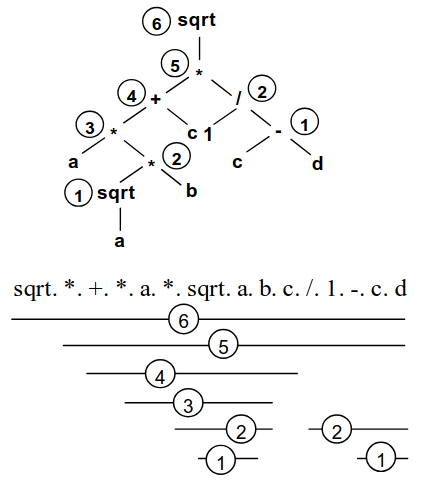
\includegraphics[width=0.5\textwidth]{Figures/chapter_gep/p_gep.png} % Include the figure image
        \caption{Illustration of hierarchy of P-GEP (\cite{li2005prefix})}
        \label{fig:p_gep} % Unique label used for referencing the figure in-text
\end{figure}

\noindent \textit{S\_GEP}, an extension of \textit{P-GEP}, has a unique characteristic to overcome the above shortcomings, which is its ability to evaluate the linear chromosomes using a stack (\cite{peng2014improved}). In order to evaluate the chromosome using a stack, the effective length of the gene needs to be calculated which represents the coding region. The effective gene length, \textit{el}, is calculated as shown in Algorithm \ref{alg:effective_length}.

\parbreak\noindent The effective gene length can then be used to evaluate the chromosome using a stack which is then visualized in Figure \ref{fig:gep_stack}. The effective gene is read in Polish notation fashion whereby the symbols are read right to left. As terminals are read, they are pushed onto the stack, and when a function symbol is encountered, it takes the terminals on the stack as input. The result is then pushed back on the stack and the process repeated until a single result remains. This mechanism can be summarized using Algorithm \ref{alg:gep_stack}.

\parbreak
\begin{algorithm}
	\caption{Effective gene length (adapted from \cite{peng2014improved})}\label{alg:effective_length}
	\begin{algorithmic}[1]
	% \Ensure $y = x^n$
	\item \textbf{Input}: String of gene symbols
	\item \textbf{Output}: eL
	\item Initialize variables $Len=1$ and $count=0$
	\item \textbf{while} scanning gene symbols starting from left to right
	\item \quad $Len = Len + 1$;
	\item \quad \textbf{if} current gene symbol is function:
	\item \quad \quad $count = count - 1$
	\item \quad \textbf{else}:
	\item \quad \quad $count = count - 1$
	\item \quad \textbf{if} $count < 0$
	\item \quad \quad return $eL=Len$ as output
\end{algorithmic}
\end{algorithm}

\parbreak
\begin{figure}[H] % Use [H] to suppress floating and place the figure/table exactly where it is specified in the text
    \centering % Horizontally center the figure on the page
    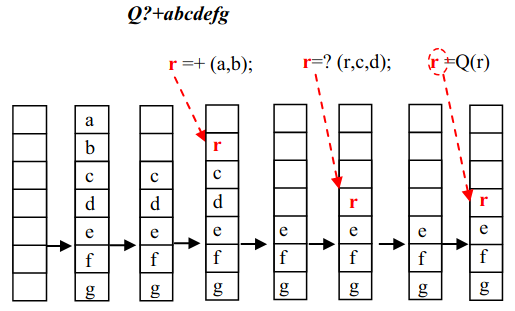
\includegraphics[width=0.75\textwidth]{Figures/chapter_gep/gep_stack.png} % Include the figure image
    \caption{Evaluation of GEP chromosome using stack (\cite{peng2014improved})}
    \label{fig:gep_stack} % Unique label used for referencing the figure in-text
\end{figure}

\parbreak\noindent \textit{S\_GEP} proved to show favourable results by outperforming traditional GEP in terms of its computation efficiency (\cite{peng2014improved}). Although applied primarily to regression problems, \textit{S\_GEP} poses as a powerful technique in general application, however, in the context of this research, GEP-NN specifically.

\parbreak
\begin{algorithm}
	\caption{S\_GEP Algorithm (adapted from \cite{peng2014improved})}\label{alg:gep_stack}
	\begin{algorithmic}[1]
	\item Calculate eL using Algorithm \ref{alg:effective_length}
	\item \textbf{while} reading effective gene from right to left using eL
	\item \quad \textbf{if} current gene is a terminal symbol:
	\item \quad \quad push terminal symbol on stack
	\item \quad \textbf{else if} current gene is function symbol:
	\item \quad \quad pull terminal symbols from stack and feed to function symbol
	\item \quad \quad push result value to stack
	\item pull value from stack and return
\end{algorithmic}
\end{algorithm}